%!TEX root = ../../main.tex


\begin{figure}[!tbp]
\centering
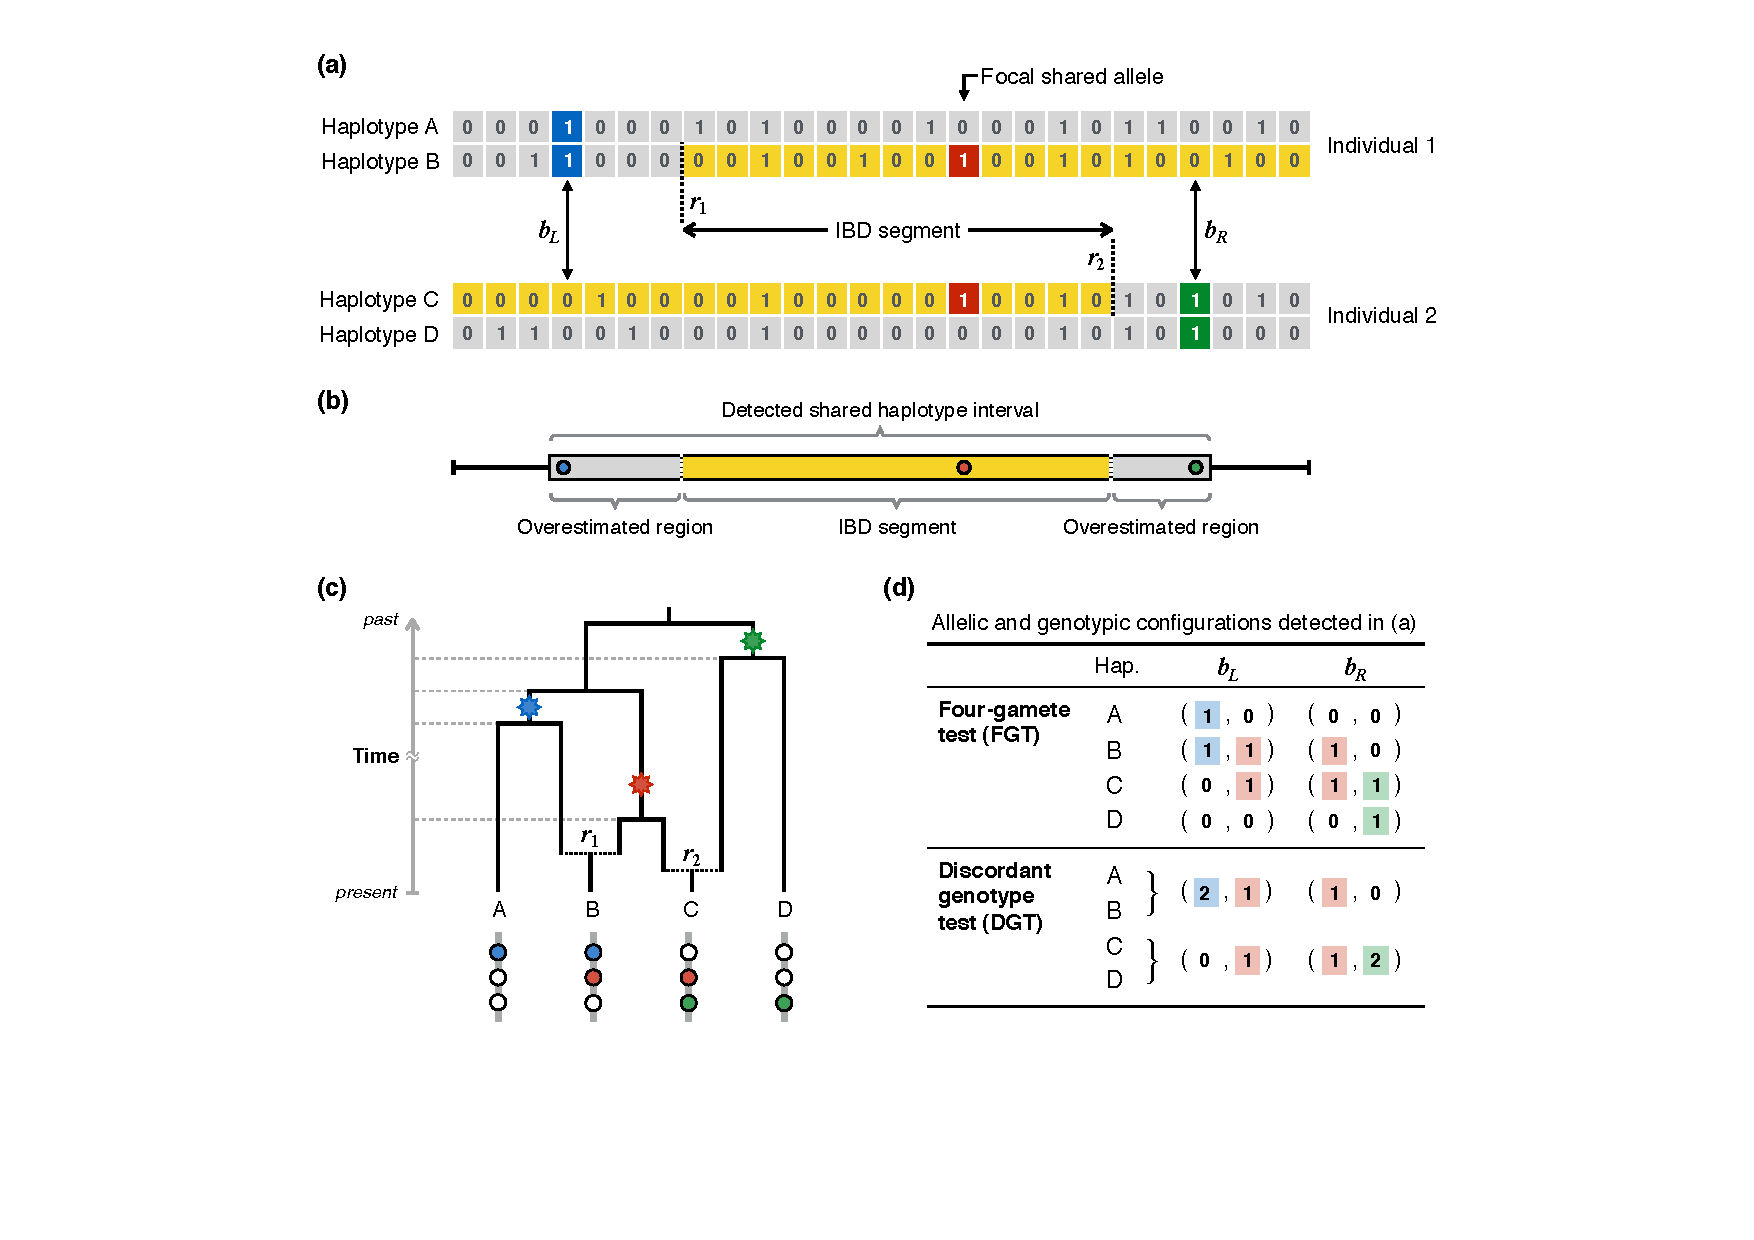
\includegraphics[width=\textwidth]{./img/ch3/info_breakpoint}
\Caption{Illustration of shared haplotype detection in a pair of diploid individuals}
{Panel~\textbf{(a)} shows \n{2} individuals composed of haplotypes A and B, and haplotypes C and D, respectively.
Each haplotype is represented as a sequence of observed allelic states, where $0$ and $1$ denote the ancestral and derived allele, respectively.
Breakpoints are detected by independently scanning to the left and right-hand side from the target position.
The \n{2} individuals share a haplotype by descent (highlighted in \emph{yellow}) which is tagged by the focal allele (\emph{red}), for which the \n{2} individuals are heterozygous
\N{2} sites (\emph{blue} and \emph{green}) mark the first sites at which a breakpoint condition is satisfied, such that $b_{L}$ and $b_{R}$ are detected.
The IBD segment shared by both individuals is indicated by $r_{1}$ and $r_{2}$ (\emph{dashed lines}).
Panel~\textbf{(b)} shows the detected breakpoint interval, delimited by $b_{L}$ and $b_{R}$ (inclusive).
Note that detected breakpoints are only the first indication of recombination found distal to the focal site, but may not mark the points of the actual crossover events; thus, it is expected that the length of the detected segment is overestimated, dependent on available data.
Panel~\textbf{(c)} represents the history of the sample as an \gls{arg}.
Mutation events are indicated on the tree (\emph{stars}) and gave rise to the alleles highlighted in~(a); \emph{blue}, \emph{red}, and \emph{green}.
The dotted \emph{grey} lines indicate the time of coalescent events in the history of the sample; dotted \emph{black} lines indicate recombination events.
Panel~\textbf{(d)} provides a table outlining the configurations of allelic and genotypic states at breakpoint sites as considered in the \gls{fgt} and \gls{dgt}, respectively.
Notably, in the example shown, both the \gls{fgt} and \gls{dgt} detect breakpoints at indicated sites.
But, for example, if individual~1 was composed of haplotypes A and C, and individual~2 of haplotypes B and D, the breakpoints would be detected as shown under the \gls{fgt}, but not the \gls{dgt}.}
{fig:info_breakpoint}
\end{figure}
